\documentclass{trbunofficial}

% import encoding and font packages for pdflatex, in order 
\usepackage[T1]{fontenc}    % output T1 font encoding (8-bit) so accented characters are a single glyph
\usepackage[utf8]{inputenc} % allow input of utf-8 encoded characters

% import language and regionalization packages, in order
\usepackage[strict,autostyle]{csquotes} % smart and nestable quote marks
\usepackage[USenglish]{babel}           % automatically regionalize hyphens, quote marks, etc
\usepackage{microtype}                  % improves text appearance with kerning, etc
\usepackage{booktabs}
\usepackage{graphicx}

% \usepackage[colorlinks=true,linkcolor=blue,citecolor=blue]{hyperref}
% For TRB version hide links
\usepackage[hidelinks]{hyperref}

% Put here what will go to headers as author
\AuthorHeaders{Boeing and Riggs}
\title{Converting One-Way Streets to Two-Way Streets to Improve Transportation Network Efficiency and Reduce Vehicle Distance Traveled and Emissions}

\author{%
  \textbf{Geoff Boeing}\\
  Department of Urban Planning and Spatial Analysis\\
  Sol Price School of Public Policy\\
  University of Southern California\\
  Los Angeles, California, USA\\
  ORCID: 0000-0003-1851-6411\\
  Email: boeing@usc.edu\\
  \hfill\break% this is a way to add line numbering on empty line
  \textbf{William Riggs}\\
  Department of Public and Nonprofit Administration\\
  School of Management\\
  University of San Francisco\\
  San Francisco, California, USA\\
  ORCID: 0000-0001-8562-5998\\
  Email: wriggs@usfca.edu
}

% If necessary modify the number of words per table or figure default is set to
% 250 words per table and figure
\setcounter{wordspertable}{250}
\setcounter{wordsperfigure}{0}

% If words are counted manually, put that number here. This does not include
% figures and tables. This can also be used to avoid problems with texcount
% program i.e. if one does not have it installed.
\setcounter{textwords}{6031}

\begin{document}
\maketitle

\section{Abstract}

The social, safety, and economic benefits of converting one-way streets to two-way streets have been documented recently in the urban planning research literature. However, it is less-understood how these conversions could impact environmental quality---including vehicle kilometers traveled (VKT), fuel consumption, and greenhouse gas emissions. Hypothetically, all three outcomes could decrease as two-way streets unlock more flexible use of transportation networks and more direct routing. Focusing on the city of San Francisco, this study builds on past work exploring network efficiency and analyzes the impacts of two-way street conversion on shortest-path trip distances. We find that the average trip in the current real-world network (with one-way streets) is about 1.5\% longer than it would be in an alternative network with all bidirectional streets. This surplus travel to navigate directionality restrictions corresponds, per year for intra-city trips, to an estimated extra 24 million kilometers traveled, 2.3 million liters of gasoline consumed, and 5.5 million kilograms of carbon dioxide released. The presence of one-way streets fundamentally limits the extent to which motorists can choose to minimize VKT: if San Francisco's one-way streets were made bidirectional, we estimate that motorists who seek to minimize VKT could reduce theirs by 1.46\% through new network efficiency. These findings illustrate the trade-offs that politicians, planners, and engineers face in aligning local policy, finance, and street design goals with climate-oriented objectives.

\hfill\break%
\noindent\textit{Keywords}: environmental quality, street conversion, transportation policy, urban design
\newpage

\section{Introduction}

The past few years have witnessed much discussion of the benefits of converting one-way urban streets to two-way. Research has shown that two-way streets can improve network function \cite{gayah_two-way_2012,gayah_analytical_2012} and be safer and more livable than one-way corridors \cite{riggs_two-way_2016}. Urban designers have amplified this work to discuss the place-making value of slower and safer streets that support multimodal travel. As a result, many cities are rethinking how urban streets should be designed and considering conversions of one-way corridors to promote safety and economic goals as large segments of the population return to live in urban areas. This rethinking involves renovating streets of urban neighborhoods, which have suffered from years of neglect because of a focus on suburban development \cite{dover_street_2013,duany_suburban_2001}. It also involves consideration of how new mobility and micro-mobility advances are changing travel behavior and patterns in cities \cite{clewlow_disruptive_2017,clewlow_micro-mobility_2018,riggs_disruptive_2019,shaheen_shared_2018}.

While these broader benefits have gained some degree of consensus in the academic literature, narrower considerations of vehicular flow are more mixed. On one hand, one-way streets were originally designed to accelerate vehicles through automobile-oriented rights of way with simplified, efficient intersections. Yet there is more to efficiency than just this. One critical aspect is that, mathematically, a shortest-path between two points in a fully bidirectional network may be shorter than than the shortest-path between these same points in a network with some one-ways, but the opposite is never true \cite{ortigosa_analysis_2019}. This is because one-way streets sometimes force drivers to divert several blocks out of their way to overcome the directionality restrictions and arrive at their destination. While planners have explored the livability and economic benefits of two-way street conversions, and engineers have explored their flow-efficiency impacts, an important research gap currently exists: it is not well-understood how these conversions could impact vehicle kilometers traveled (VKT), fuel consumption, and greenhouse gas (GHG) emissions. All of these outcomes could hypothetically decrease as two-way streets allow for more direct automobile routing, but to what extent would this be the case given real-world network geometry and topology?

This paper takes preliminary empirical steps to better understand one-way to two-way street conversions' impacts on transportation network efficiency, travel, and emissions. We construct two network models to simulate the efficiency of the drivable street network of the city of San Francisco. The first (\enquote{as-is}) model preserves real-world one-way driving constraints, while the second (\enquote{as-proposed}) model treats every street as bidirectional. We then use California Household Travel Survey (CHTS) home/workplace coordinates to generate commute origins and destinations, then simulate trips on each of the two networks. Comparing the resulting trips, we find that two-way streets allow for significantly shorter travel distances and potentially lower fuel consumption and emissions. This provides a stronger political and engineering argument for these street conversions beyond recent public health and economic development arguments.

This paper is organized as follows. The next section surveys the recent research literature around one-way/two-way street conversions. Then we explain the details of our methodology and present the empirical results. Finally, we discuss these findings and potential implications for transportation policy.

\section{Background}

\subsection{The Logic of One-Way Streets}

Essentially all city streets historically allowed bidirectional traffic flows. Between the 1950s and 1980s, many cities converted two-way streets to one-ways to promote traffic flow to burgeoning post-war suburbs for an increasingly automobile-centric, mid-century population \cite{appleyard_livable_1980,hall_cities_1996,handy_planning_2003,jackson_crabgrass_1987}. The logic of these streets was centered around having a central destination for employment with an inflow and outflow of jobs. In this monocentric vision of the city, one-way streets optimized high capacity vehicular flow from one point to another, facilitating higher traffic volumes and centrifugal urbanization \cite{dover_street_2013}. City engineers designed roadways to maximize inflow and outflow, irrespective of distance, with hierarchies built for the emerging settlement patterns of the time---automobile-dependent suburban neighborhoods \cite{buchanan_traffic_1963,bavarez_traffic_1967}. The combination of streets (inclusive of one-way couplets) enabled higher travel speeds, over longer distances, with less frequent stops for vehicles \cite{hebbert_engineering_2005}.

The glorification of the heavily-engineered street optimized for vehicular traffic remains pervasive today. Yet it increasingly comes into conflict with other evolving goals of urban planning and design. A tension arises between humans moving quickly across cities and humans accessing and spending time in places \cite{hebbert_engineering_2005}. City planners today increasingly emphasize compact development, density, environmental sustainability, and land use diversity \cite{stevens_does_2017,salon_how_2012}. One-way---and reciprocally, two-way---streets play an important role in these debates.

\subsection{The Argument for Two-Way Streets}

The impacts of 20th century shifts in street design to promote automobile-oriented suburban expansion---and efforts to rethink them---have been the subject of substantial discussion in recent planning research. Researchers have found that these two-way to one-way conversions (and subsequent changes in adjacent land use) resulted in disinvestment and a degraded street-level human experience \cite{cervero_travel_1997,leinberger_walk_2012}. A large body of work provides evidence that dense urban networks with a diversity of land uses promote more sustainable and diverse commute modes \cite{ewing_travel_2010,frank_many_2006,frederick_commute_2018}. From the practitioner's perspective, \citet{speck_walkable_2018} recently identified 78 cities that successfully restored one-way streets back to two-way, and at substantially lower costs than anticipated. The financial feasibility is also supported by a larger body of work identifying the life-cycle cost effectiveness of roadway and traffic-calming changes \cite{noland_costs_2015}.

The literature also includes research on the potential of street conversions to support livability, equity, and economic goals \cite{riggs_two-way_2016,riggs_economic_2017, riggs_economic_2018}. Instead of reinforcing automobile level-of-service (LOS) and vehicular flow as the supreme aims of transportation planning, this body of research recognizes the importance of a more comprehensive approach to urban quality of life. It demonstrates how changes to the urban right-of-way can support urban regeneration and revitalization. For instance, \citet{riggs_two-way_2016} find that two-way streets create higher levels of economic activity compared to one-way streets because they give drivers more exposure to local businesses and provide local business exposure to individuals traveling in two directions versus those traveling in only one.

Another major research topic has been safety. While the engineering literature has tended to focus on first-order effects (such as LOS), equal attention should be paid to second-order effects. One-way streets may lead to higher speeds \cite{schneider_pedestrian_2013}, which may be desirable from an LOS or vehicular-throughput perspective, but other scholars have found that this is accompanied by an increased risk to pedestrian safety \cite{swift_residential_1998} and a false sense of security for drivers \cite{holahan_psychological_2013}. Several studies have found that one-way streets are often less safe than their two-way counterparts \cite{ewing_urban_2003,riggs_two-way_2016,ewing_built_2009}. Although some research suggests that older adults may struggle crossing two-way streets \cite{dommes_functional_2013}, broader longitudinal work suggests that one-way streets are less safe for children \cite{wazana_are_2000}: children are 2.5 times more likely to have a pedestrian injury on a one-way versus two-way street. \citet{gayah_two-way_2012} and \citet{gayah_analytical_2012} argue that two-way streets are safer for pedestrians because their greater complexity requires motorists to drive more attentively and slowly, and vehicular-pedestrian conflict points are more easily anticipated. Two-way streets are also easier to navigate and less confusing than one-way streets, especially for visitors to a new area.

\begin{figure*}[tbp]
	\centering
	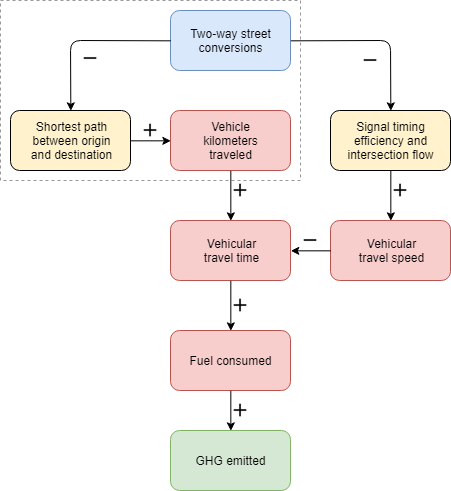
\includegraphics[width=0.5\textwidth]{figures/conversions_ghg.png}
	\caption{Theoretical model of one-way to two-way street conversions' effects on vehicle travel, fuel consumption, and emissions.}
	\label{fig:conversions_ghg}
\end{figure*}

\subsection{Re-Thinking Conversions' Effects}

Today, the research literature advocating for conversions back to two-way streets tends to focus on social and safety benefits. Meanwhile, the engineering literature demonstrating the superiority of one-way streets tends to focus on efficiency benefits, emphasizing signal timing and intersection flow, but not on the composition of the city. This is only part of the picture. Two-way conversions may offer a different set of network efficiency gains by reducing shortest-path distances along the network. Figure \ref{fig:conversions_ghg} presents a theoretical path model (represented as a directed acyclic graph) of how two-way street conversions impact vehicle travel, fuel consumption, and emissions. The two primary network policy and design (in-)efficiencies are highlighted in yellow. Past research has focused on the right-side pathway, emphasizing one-way streets' positive benefits on signal timing and roadway throughput.

Less is currently known about the left-side pathway's impact on VKT (delimited by the dashed gray bounding box). Yet reducing VKT, and in turn fuel consumption and emissions, is critical to achieving urban climate goals \cite{barrington-leigh_more_2017}. \citet{ortigosa_analysis_2019} argue that two-way networks could theoretically reduce VKT because they can provide drivers more direct routes from one location to another, while one-way street networks increase the average driving distance. Although they can exhibit fewer stop-and-go effects at intersections due to signal timing, one-way street networks are less efficient from a distance-traveled standpoint. However, like much of this body of work, this relies on abstract models to make theoretical claims about idealized networks. Little empirical work with real-world case studies has been done on this left-side pathway. 

\section{Methods}

This paper takes up this research gap and asks: to what extent do one-way restrictions increase shortest-path distances in a real-world city street network? Building our knowledge of the left-side pathway (Figure \ref{fig:conversions_ghg}), it advances the body of research on the efficiency of two-way networks by making three contributions. First, it builds on the theoretical model of \citet{ortigosa_analysis_2019} by conducting an empirical real-world case study of San Francisco's street network. Second, it explores distance-traveled through both a randomized set of origins/destinations (OD) and a survey-derived set to investigate network performance from different perspectives. Third, it supplements the distance-traveled analysis with a preliminary \textit{ceteris paribus} estimation of surplus fuel consumption and GHG emissions, adding a new environmental-impact dimension to the policy analysis research literature.

We construct two models of the city of San Francisco's drivable street network using data from OpenStreetMap. We choose San Francisco as a case study because it is reasonably large and reasonably representative of many US urban circulation systems: it contains a variety of neighborhoods with different network patterns and includes both one-way and two-way streets, like most large US cities. OpenStreetMap is a worldwide collaborative mapping project and platform that anyone can contribute to \cite{jokar_arsanjani_openstreetmap_2015}. Its data are high-quality and detailed, providing a good source for modeling and analyzing transportation networks \cite{barron_comprehensive_2014,zielstra_assessing_2013,barrington-leigh_worlds_2017,zhao_agent-based_2019}. For each model, we download the drivable street network in the city of San Francisco using OSMnx, a Python-based toolkit for automatically downloading, modeling, and analyzing city street networks using OpenStreetMap data \cite{boeing_osmnx:_2017,boeing_multi-scale_2018,boeing_street_2019}. We then filter out freeways to construct two models of the surface street network in the city. The first model preserves real-world one-way directionality constraints by modeling the network as a directed graph, $G_1$. The second model treats every street as bidirectional, using an undirected graph, $G_2$. Both graphs are topologically defined such that vertices represent intersections and dead-ends, and edges represent the street segments that link them.

Next we construct two OD matrices to represent trip endpoints. For the first matrix, we use the CHTS to generate an $n \times 2$ \enquote{survey-derived} OD matrix $M_s$, where $n$ equals the number of daily vehicle trips (i.e., 1,133,333) that begin and end in San Francisco \cite{san_francisco_county_transportation_authority_tncs_2017}, which is spatially representative of the actual origins (homes) and destinations (workplaces) for each household in the survey with both home and work within the city limits. For the second matrix, we randomly select $n$ origin and destination nodes from the graph to generate a \enquote{randomized} OD matrix $M_r$ of dimension $n \times 2$. This second matrix provides a robustness test for the first to 1) corroborate that the simulated estimates are in the same range across both OD matrices, and 2) to cover different sections of the city more-evenly than home-work commutes alone might.

Next we simulate all of the trips in each of the OD matrices on each of the two graphs, using two implementations of Dijkstra's shortest-path algorithm. The first algorithmic implementation, $A_1$, uses no weights and counts the topological distance (i.e., number of edges, which corresponds to the number of linear blocks) traversed on the shortest path between the origin and destination. The second implementation, $A_2$, weights edges by length, to minimize total distance traveled. Both assume free-flow travel without a queuing model. Finally, we analyze the differences in trips (for both OD matrices) between the two graphs to compare cumulative travel on the real-world network with one-way streets versus the alternative model with all bidirectional streets.

\section{Results}

First we examine the number of blocks traversed given randomized origins and destinations. Using OD matrix $M_r$ and implementation $A_1$, we find that the typical (median) trip on $G_1$ must traverse 3 additional blocks (edges) compared to the typical trip on $G_2$ (49 edges versus 46 edges). We conduct a difference-in-means $t$-test and find the average (mean) trip traverses statistically-significantly more blocks on $G_1$ than on $G_2$: the difference in means is 2.57 blocks ($t=91.20$, $p<0.0001$).

Next we examine the distance traveled given randomized origins and destinations. Using OD matrix $M_r$ and implementation $A_2$, the typical trip on $G_1$ travels a distance of 6,448 meters while the typical trip on $G_2$ travels 6,363 meters. Thus, the typical trip on $G_1$ yields about 1.3\% more VKT than that on $G_2$. We conduct a difference-in-means $t$-test and find the average (mean) trip is statistically-significantly longer on $G_1$ than on $G_2$: the difference in means is 84 meters ($t=21.19$, $p<0.0001$).

Next we examine the number of blocks traversed given survey-derived origins and destinations. Using OD matrix $M_s$ and implementation $A_1$, we find that the typical (median) trip on $G_1$ must traverse 2 additional blocks compared to the typical trip on $G_2$ (38 edges versus 36 edges). We conduct a difference-in-means $t$-test and find the average (mean) trip traverses statistically-significantly more blocks on $G_1$ than on $G_2$: the difference in means is 1.76 blocks ($t=64.82$, $p<0.0001$).

Finally we examine the distance traveled given survey-derived origins and destinations. Using OD matrix $M_s$ and implementation $A_2$, the typical trip on $G_1$ travels a distance of 4,943 meters while the typical trip on $G_2$ travels 4,871 meters. Thus, the typical trip on $G_1$ yields about 1.5\% more VKT than that on $G_2$. We conduct a difference-in-means $t$-test and find the average (mean) trip is statistically-significantly longer on $G_1$ than on $G_2$: the difference in means is 72 meters ($t=18.91$, $p<0.0001$).


\begin{table}[tbp]
\centering
\caption{Results from simulating the trips; \enquote{surplus} rows refer to excess consumption/release on the current network with one-way streets ($G_1$) in relation to a fully-bidirectional alternative network ($G_2$), and pertain to intra-city trips only.}
\label{tab:results}
\footnotesize
\begin{tabular}{lllll}
\toprule
& \multicolumn{2}{l}{Survey-derived trips} & \multicolumn{2}{l}{Randomized trips}   \\
\midrule                                         
                                      & $G_1$      & $G_2$  & $G_1$      & $G_2$    \\
\midrule
Median trip length (m)                & 4,684      & 4,606  & 6,330      & 6,235    \\
Mean trip length (m)                  & 4,943      & 4,871  & 6,448      & 6,364    \\
Median blocks traversed               & 38         & 36     & 49         & 46       \\
Mean blocks traversed                 & 39.0       & 37.2   & 49.8       & 47.3     \\
Surplus annual VKT                    & 24,247,315 & ---    & 21,878,100 & ---      \\
Surplus annual fuel consumed (liters) & 2,309,035  & ---    & 2,083,418  & ---      \\
Surplus annual CO2 released (kg)      & 5,533,650  & ---    & 4,992,955  & ---      \\
\bottomrule
\end{tabular}
\end{table}


How does this estimated surplus travel impact fuel consumption and GHG emissions? Focusing on OD matrix $M_s$ (because it best reflects real-world parameterization), the average trip in the real-world network (with one-way streets) is about 1.5\% longer than that of the proposed alternative network (with all bidirectional streets). This difference is statistically significant but it is also practically significant: given the San Francisco County Transportation Authority's estimates of real-world daily VKT for trips that begin and end within the city \cite{san_francisco_county_transportation_authority_tncs_2017}, we estimate that the presence of one-way streets increases this daily VKT by more than 66,000 surplus kilometers and in turn increases annual VKT by over 24 million surplus kilometers.

Conservatively assuming an average US fuel economy of 10.5 km/liter \cite{shepherdson_u.s._2018} and average GHG emissions of 2.4 kilograms per combusted liter \cite{us_department_of_energy_how_2018}, this estimated excess travel to accommodate one-way driving restrictions expends a surplus 2.3 million liters of gasoline per year, in turn releasing an extra 5.5 million kilograms of carbon dioxide into the atmosphere---just for trips taken entirely within the city of San Francisco alone.


\section{Discussion}

Let us briefly summarize these findings. Simulating all the daily trips that begin and end within the city of San Francisco, we estimate that the presence of one-way streets increases the average shortest-path route by approximately 1.5\%. Drivers may seek to minimize various factors when choosing a route, but the presence of one-way streets places a fundamental limit on the extent to which they can even choose to minimize VKT. To put this another way, if these one-way streets were converted to two-way streets, environmentally conscious motorists (of which there are many in San Francisco) who seek to minimize their VKT could reduce their annual VKT by 1.46\%, just through new network efficiency gains.

In turn, a citywide two-way conversion policy could reduce annual VKT by 24 million kilometers, fuel consumption by 2.3 million liters, and carbon dioxide emissions by 5.5 million kilograms---just for intra-city trips that begin and end within San Francisco proper. The total impact of regional trips passing through this city would be far greater. For instance, CalTrans estimates that the total daily VKT of trips through the city is about 3.4-times greater than SFCTA's estimate of intra-city trips \cite{caltrans_2017_2018}. Given the relative consilience of the estimates produced by our survey-derived and randomized simulations, one could apply this factor to get a rough estimate of the VKT, fuel consumption, and GHG impacts of one-way streets across all trips on San Francisco's roads.

What does this mean to planning research and practice? First and foremost, these results provide a new and more nuanced understanding of the trade-offs that planners face in roadway design (i.e., prioritizing one-way vehicular efficiency at the cost of safety, livability, VKT, fuel consumption, and GHG emissions). A predominant assumption in roadway design over the past half-century has been that one-way streets offer more efficient traffic flow. While there are many theoretical models to predict driver routing, these findings demonstrate a fundamental inherent network inefficiency to one-way streets, with significant VKT and GHG ramifications. One-way streets force cars to 1) traverse additional blocks and distance, 2) consume surplus fossil fuel to accommodate this necessitated excess travel, and 3) in turn, emit millions of kilograms of surplus GHGs. While one-way networks can offer signal timing and intersection efficiencies, they produce other inefficiencies.

These results thus contribute to the bigger-picture dialogue. In 2017 Stevens \cite{stevens_does_2017} published a paper in the Journal of the American Planning Association suggesting that planners and engineers tend to over-estimate the benefit of compact development, and that they \enquote{should probably assume for now that... [it] will have a small influence on driving... and municipal decision makers should not rely on compact development as their only strategy for reducing VMT.} While this approach was, in turn, critiqued by Handy \cite{handy_thoughts_2017} who argued that planning and engineering professionals cannot sufficiently reduce driving and address climate-related goals without compact development, there have been few other strategies discussed in the literature that can help impact VKT reduction at scale. One-way street conversions offer a straightforward tool in the planner's and policymaker's toolkit to address the looming climate crisis. Street conversions are not without costs, but failing to address climate goals proactively could be far more costly. Moreover, the costs of conversion are further attenuated by the livability and economic benefits of two-way streets, apart from VKT-efficiency.

This study demonstrates that there may be more benefits to street conversion than merely improved access, safety, livability, and economic conditions--—they also allow drivers to optimize for less VKT and consequent emissions. While these climate impacts vary for travelers from different parts of a city, and we do not directly measure changes in vehicular LOS at a neighborhood level, they would be likely be visible at that level: local travel would become more efficient as there would be less circling behavior and less traveling around blocks unnecessarily to get to destinations. In networks with short streets and high congestion levels, two-way networks offer a better spread of the congestion than one-way networks, are less likely to reach gridlock, and allow for lower VKT. Conversions offer a straightforward engineering solution that can yield these benefits, alongside the many other social benefits recently identified by researchers.

This preliminary work stimulates a number of new research questions and next steps. First, one-way streets are an embedded part of many cities' infrastructure, which could raise concerns about high conversion costs. The research literature has documented many benefits to conversion and we have identified new benefits in this study---but are they worth the cost? Fortunately, research has shown that street conversions are usually less costly than expected, particularly when evaluated over the life-cycle of an asset, and can bring the ancillary economic development benefits discussed in the background section \cite{speck_walkable_2018,riggs_two-way_2016,steuteville_cities_2019,noland_costs_2015}. Future research should conduct a detailed cost-benefit analysis, weighing conversion's benefits of livability, safety, economic development, and reduced VKT/GHG against financial costs and vehicular LOS (which itself comes at a substantial social cost).

Second, and related, this paper focused on the left-side pathway in Figure \ref{fig:conversions_ghg} to empirically demonstrate real-world impacts on VKT minimization. This preliminary analysis was conducted \textit{ceteris paribus}---it did not allow for simultaneous changes in the right-side pathway. Future work should model the various network distance and throughput effects through the multiple pathways of shortest-paths, signal timing, intersection flow, and queuing. A comprehensive such model would be complex, and outside the scope of this present project investigating the left-side pathway empirically for the first time, but it would be important for better understanding productivity gains and time savings that ultimately could yield additional economic value. As vehicles automate and gain networking capacity in themselves, policy/design optimizations that allow algorithms to minimize distance traveled would remain invariant and important.

Finally, future work should expand these empirical findings by modeling and simulating two-way conversions effects at multiple scales: neighborhood, municipality, and region. This should also compare and contrast cities in different parts of the country to better understand the regional variation or importance of these policy and design changes.

\section{Conclusion}

Substantial recent urban policy/design research highlights the social benefits of converting one-way streets to two-way streets. Yet much of today's road engineering research and practice instead emphasize vehicular efficiency, through measures like LOS, that preference one-way streets. The latter usually focuses on signal timing and intersection flow, but less was known empirically about two-way conversions impacts on shortest-path distances in real-world networks.

This study addressed this gap by modeling San Francisco's street network and simulating trips along \enquote{as-is} versus fully-bidirectional model variants. We found that one-way streets fundamentally limit motorists' ability to minimize VKT. If San Francisco's one-way streets were converted to two-way streets, motorists could reduce their VKT by nearly 1.5\%, which would correspond to an annual reduction of 24 million VKT, 2.3 million liters of fuel, and 5.5 million kilograms of carbon dioxide---just for intra-city trips alone.

These findings provide planners and policymakers with a new rationale for considering these street engineering projects. One-way to two-way conversions come with costs (both financial, and vehicular LOS), but they should be considered after a careful accounting of the \textit{full} social and environmental benefits. Cities ranging from South Bend, Indiana and Klamath Falls, Oregon to Austin, Texas and Denver, Colorado have recently engaged in conversions, our work suggests that more cities should consider their ancillary benefits. We argue that there are broader political and engineering arguments for these projects beyond the recent public health and economic development arguments. While conversions have financial and political costs, they can provide small but quick wins for cities fighting climate change--—a straightforward local policy and engineering shift with a climate-oriented benefit. 


\bibliographystyle{trb}
\bibliography{references}
\end{document}
